\chapter{State of the Art}\label{sec:chap:2}

\section{Software Defined Networking}\label{sec:chap2_sdn}

Software Defined Networking (SDN) is an approach to networking that revolves around the abstraction between the forwarding and control planes. This facilitates programmatically control over the network in order to operate network services in a deterministic, dynamic and scalable manner \cite{rfc_7426}.\\

SDN is part of a long history of efforts to make computer networks more programmable, going back more than twenty years. SDN shares simmilarities with early telephony networks, where there was a clear separation between control and data planes to simplify network management and the deployment of new services \cite{road_to_sdn}.\\

By centralizing the network control, SDN offers flexibility to congfigure, manage, secure, and optimize network resources via dynamic SDN programs that can be programed independently of the implementation of the network. SDN makes it possible to manage the entire network through intelligent orchestration \cite{new_norm_sdn}.\\

Figure 1 offers a logical representation of the SDN architecture. The Network inteligence resides in the controller, a software-based centralized SDN entity with a global view of the network. APIs between the application layer and the control layer offer the possibility of introducing applications that operate on an abstracion of the network regardless of the details of the implementation.

\begin{center}
\begin{figure}[h!]
  \centering
    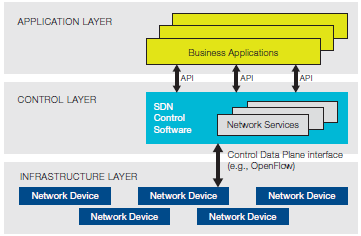
\includegraphics[scale=0.9]{./images/openflowjason}
	\caption{Openflow Logical Representation}
	\label{openflow-fig}
\end{figure}
\end{center}

\subsection{OpenFlow}\label{sec:chap2_sdn_openflow}

The Open Networking Foundation (ONF) is a non-profit organisation that is leading the development of SDN, including the standardisation of the OpenFlow protocol. OpenFlow provides the communication between the control and data planes and is the first standard interface designed specifically for SDN. Some of the benefits OpenFlow-based SDN offer to enterprises and carriers are:

\begin{itemize}
\item{\textbf{Centralized management and control of multi-vendor environments:} SDN control software can control any OpenFlow-enabled device.}
\item{\textbf{Reduced complexity through automation:} OpenFlow-based SDN offers a flexible network automation and management framework.}
\item{\textbf{Higher rate of innovation:} Due to the capacity of network operators to program te network in real time to meet specific needs in a short frame of time.}
\item{\textbf{Increased network reliability and security:} Due to the complete visibility and control of the network from a centralized entity.}
\item{\textbf{More granular network control:} Capability of setting low level network parameters at a high level.}
\item{\textbf{Better end-user experience:} Due to network behaviour adapting to the user's needs, using state information being available to higher-level applications.}
\end{itemize}

Both the SDN controller and the network nodes run the OpenFlow protocol. The OpenFlow protocol's key concept are flows, which identify the network traffic based on rules that are programmed at the SDN control level. These rules establish the way traffic flows through the network through the diffent network nodes that form it.

\subsubsection{OpenFlow Switch}\label{sec:chap2_sdn_openflow_switch}

An OpenFlow Switch is a software program or hardware device that consists at least of a Flow Table, an Action associated with each Flow Table Entry and an OpenFlow Secure Channel. The Flow Table performs packet lookups and forwarding, and the OpenFlow Secure Channel connects the OpenFlow switch with the SDN Controller. The switch communicates with the controller and the controllwer manges the switch via the OpenFlow protocol \cite{of_switch_spec}. Figure \ref{openflowswitch-fig} depicts a logical view of the OpenFlow Switch.\\

A high percentage of today's routers and Ethernet switches run flow-tables that are usually built from TCAMs, and OpenFlow takes advantage of common functionalities they share. Exploiting this feature, the OpenFlow protocol can program the flowtable regardless of the vendor of the equipment \cite{of_campus_net}.

\begin{center}
\begin{figure}[h!]
  \centering
    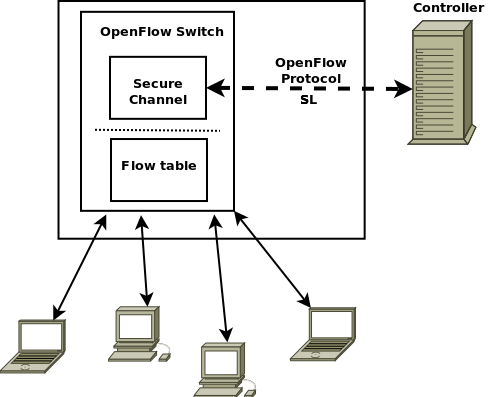
\includegraphics[scale=0.55]{./images/OpenFlowSwitch}
	\caption{OpenFlow Switch Representation}
	\label{openflowswitch-fig}
\end{figure}
\end{center}

The datapath of an OpenFlow Switch consists of a Flow Table containing three fields:

\begin{itemize}
\item{\textbf{Packet header:} Defines the flow.}
\item{\textbf{Action:} Defines how the flow should be processed.} 
\item{\textbf{Statistics:} Keeps track of the number of packets and bytes introduced by the flow and how long since the last packet for control of inactive flows.}
\end{itemize}

The three basic actions to be included in the action field of a Flow Table are:

\begin{itemize}
\item{\textbf{Forward:} In order to provide routing capabilities, this action forward packets associated to a given flow to a port or group of ports.}
\item{\textbf{Encapsulate:} This encapsulates a packet of a given flow (typically only the first packet) and sends it to the SDN controller for processing. The controller must decide if the flow should be added to the Flow Table.} 
\item{\textbf{Drop:} This commands to drop packets from a given flow. }
\end{itemize}

\section{Distrbuted Mobility Management}\label{sec:chap2_dmm}

Distributed mobility management (DMM) is an alternative to centralized mobility protocols such as Mobile IPv6, Hierarchical Mobile IPv6 and Proxy Mobile IPv6. The IETF is leading the standardization of DMM solutions. The DMM working group 
\footnote{\url{http://datatracker.ietf.org/wg/dmm/}} was formed in March 2012 to address the need for the implementation of a distributed anchoring model in mobile networks. The motivation to study and develop the DMM arquitectural paradigm resides in the following two challenges \cite{rfc_7333}: 

\begin{itemize}
\item{Mobile access to the Internet is increasing drastically. The traffic this will generate creates the need for updated requirements for data traffic delivery in mobile core networks. The ``flattening'' of mobile networks proves to work best for direct communication between closely located peers.}
\item{A study on mobility patterns suggest mobile nodes remain attached to the same point of attachment for relatively long periods of time \cite{locating_user}. IP mobility support is currently designed to always be active, resulting in an unnecessary loss of costs and resources.}
\end{itemize}

In centralized mobility management, the session and forwarding information is kept in a single centralized mobility anchor, which is in charge of forwarding the traffic to the mobile node's current location. The DMM arquitecture suggests a flat access by means of the distribution of mobility anchors in the data plane so that they are positioned nearer to the user. This optimises state information management because it avoids unnecessary mechanisms to forward traffic from an old mobility anchor to a new mobility anchor.\\

Problems that are solved with a DMM implementation are:

\begin{itemize}
\item{\textbf{Sub-optimal routes:} Since mobility anchors are fixed at the home address, this is where all traffic will arrive and must be forwarded from to the current mobile node's address. This results in longer end-to-end paths meaning higer delays. With a distributes mobility architecture, as the anchors are located at the very edge of the network, close to the user terminal, data paths tend to be shorter \cite{fama}.}
\item{\textbf{Lack of scalability:} A centralized entity in charge of maintaining mobility context information for each mobile node needs to have enough processing and routing capabilities to deal with all the mobile users' traffic simultaneously. DMM sugests distributing the load among several network entities.} 
\item{\textbf{Divergenge from network trends:} Mobile networks have an evolutionary tendency to become flatter, contrary to the approach of centralized mobility management}
\item{\textbf{Single point of failure and attack:} A centralized entity in charge of maintaining mobility context information for each mobile node means there is a unique point of failure and attack.}
\item{\textbf{Unnecessary mobility support:} IP mobility support is usually provided to all mobile nodes, even for users that will not move from the first point of attachment. This also applies to sessions that deal with mobility at an application level or applications that don't need a stable IP address during a handover to maintain session continuity.}
\end{itemize}

The two main approaches to implementing Distributed Mobility Management architectures in modern wireless networks are, on one side, transforming Mobile IPv6 into a distribution-oriented protocol, and, on the other, doing the same for Proxy IPv6. These approaches can be identified as client-based or network-based solutions respectively \cite{dmm_standard_land}:

\begin{itemize}
\item{\textbf{Client-based solution:} Based on the Mobile IPv6 protocol, this solution involves deploying multiple home agents at the edge of the network in order to distribute the mobility anchors. This is achieved through the idea that a mobile node can have assigned more than one IP address, meaning that the mobile node can have assigned a new IP address every time it visits an access network.}
\item{\textbf{Network-based solution:} Based on the Proxy IPv6 protocol, this solution suggests moving the mobility anchors to the edge of the network, and give them the capability for managing both the control and data plane seperately. The ability of managing both planes seperately offers the possibilty for optimal routing of data traffic.} 
\end{itemize}

\subsection{Mobile IPv6}\label{sec:chap2_dmm_mip}

Mobile IPv6 is a protocol that provides mobility support offering capabilities to mobile nodes so they can move from one Access Point to another without changing the mobile node's home address, the mobile node's permanent address. Without mobility support, once the mobile node leaves the home link, where the mobile node has its subnet prefix assigned (the first point of attachment), packets could not find there way to the mobile node. 

\subsubsection{Basic Operation}\label{sec:chap2_dmm_mip_bo}

\begin{center}
\begin{figure}[h!]
  \centering
    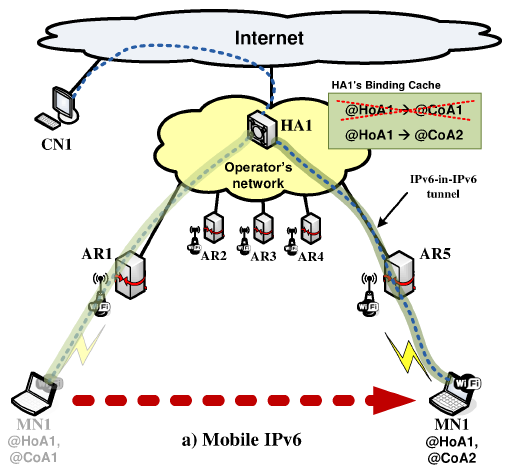
\includegraphics[scale=0.3]{./images/mip}
	\caption{Mobile IP}
	\label{mip-fig}
\end{figure}
\end{center}

More detailed information regarding the basic operation of this protocol be found in \cite{rfc_6275}.

\subsection{Proxy Mobile IPv6}\label{sec:chap2_dmm_pmip}

Mobile IPv6 poses the problem of needing the involvement of the client, having to exchange signaling messages with the home agent in order to inform of the mobile node's new location so that the home agent can redirect traffic. The Proxy Mobile IPv6 approach is a Network-based one, excluding the involvement of the host. This is possible thanks to a new entity called proxy mobility agent, that is in charge of the communication with the home agent and manange the mobility on behalf of the client.

\subsubsection{Basic Operation}\label{sec:chap2_dmm_pip_bo}

\begin{center}
\begin{figure}[h!]
  \centering
    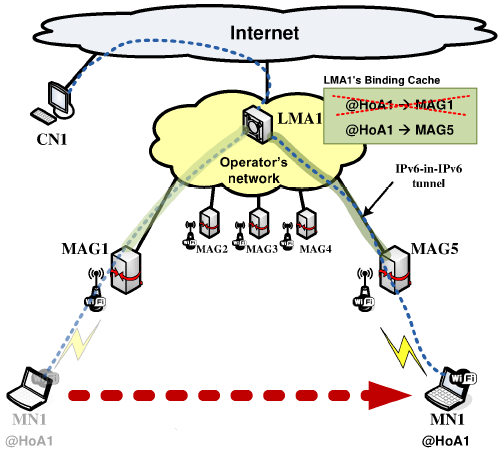
\includegraphics[scale=0.3]{./images/pmip}
	\caption{Proxy Mobile IP}
	\label{pmip-fig}
\end{figure}
\end{center}

More detailed information regarding the basic operation of this protocol be found in \cite{rfc_5213}.


\section{LTE}\label{sec:chap2_lte}

The Long Term Evolution of UMTS is the result of great technological advances in mobile telecommunications systems,standardized within the 3GPP (3\textsuperscript{rd} Generation Parnership Project) as part of the 3GPP Release 8 feature set. After the developement and standardization of GSM (Global System for Mobile communications) belonging to the 2G family, 3G  Universal Mobile Telecommunications System (UMTS) came after with the entry of Code Division Multiple Access into the 3GPP evolution track, known as Wideband CDMA (WCDMA). This technology evolved until the arrival of LTE and the adoption of Orthogonal Frequency-Division Multiplexing (OFDM), which is the access technology dominating the latest evolutions of all mobile radio standards \cite{lte_history}.\\

The LTE access network is a network of base stations called evolved NodeB (eNB), generating a flat architecture, and is the access part of the Evolved Packet System (EPS) Figure \ref{lte_arch-fig}.

\begin{center}
\begin{figure}[h!]
  \centering
    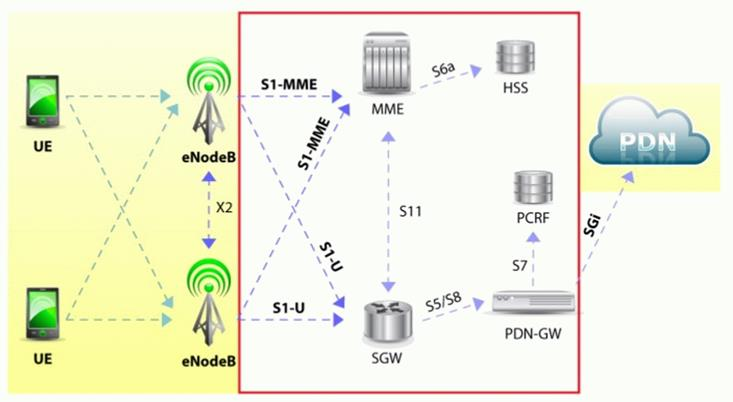
\includegraphics[scale=0.7]{./images/lte_arch}
	\caption{LTE Architecture}
	\label{lte_arch-fig}
\end{figure}
\end{center}

The latest advancements in LTE technology involve \cite{lte_wp}:

\begin{itemize}
\item{\textbf{Small Cell Enhancements}: Higher Order Modulation (256QAM) and Dual connectivity for LTE.}
\item{\textbf{Device to Device communication (D2D)}: Offerening direct and group communication between terminals.}
\item{\textbf{WLAN/3GPP Radio Internetworking}: Integration of WLAN access capabilities into  the data transfer.}
\item{\textbf{HetNet mobility enhancements}: Enhance the capacity of a cellular network by introducing heterogeneous networks (HetNets) improving overall handover performance and robustness.}
\item{\textbf{Smart Congestion Mitigation (SCM)}: For congestion control.}
\end{itemize}

\subsection{LTE emulation}\label{sec:chap2_lte_emu}

LTE emulation can be perfomed with a combination of ns-3, a discrete event network simulator used to create an open simulation environment for computer networking research and NI PXI systems \cite{ni_pxi_wp} (Figure \ref{pxi-fig}).

\begin{center}
\begin{figure}[h!]
  \centering
    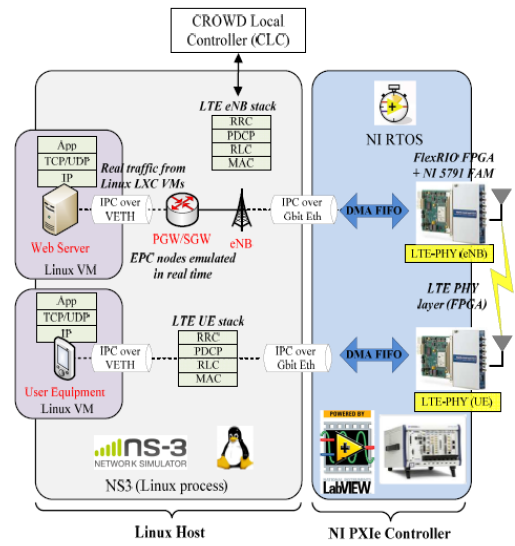
\includegraphics[scale=0.7]{./images/pxi}
	\caption{LTE emulation with ns-3 and NI PXI}
	\label{pxi-fig}
\end{figure}
\end{center}

\subsubsection{NI PXI}\label{sec:chap2_lte_emu_pxi}

PXI is a rugged PC-based platform for measurement and automation systems. PXI combines PCI electrical-bus features with the modular, Eurocard packaging of CompactPCI and then adds specialized synchronization buses and key software features. PXI is both a high-performance and low-cost deployment platform for applications such as manufacturing test, military and aerospace, machine monitoring, automotive, and industrial test. Developed in 1997 and launched in 1998, PXI is an open industry standard governed by the PXI Systems Alliance (PXISA), a group of more than 70 companies chartered to promote the PXI standard, ensure interoperability, and maintain the PXI specification \cite{ni_pxi_whatis}.

\subsubsection{ns-3}\label{sec:chap2_lte_emu_ns3}

ns-3 is a discrete-event network simulator, targeted primarily for research and educational use. ns-3 is free software, licensed under the GNU GPLv2 license, and is publicly available for research, development, and use.
The goal of the ns-3 project is to develop a preferred, open simulation environment for networking research: it should be aligned with the simulation needs of modern networking research and should encourage community contribution, peer review, and validation of the software \cite{ns3_whatis}.















